%-------------------------------------------------------------------------
%	Chaos and Quantum Chaos, Benjamin Wolba
%-------------------------------------------------------------------------

\documentclass{article}

\addbibresource{Ref_Lyapunov.bib} 										    % integration of .bib-file

\title{Notes on Lyapunov Exponents}  
\author{Benjamin Wolba}


\begin{document}

\maketitle


\section{Introduction}

Lyapunov exponents aim to quantify the term "\textbf{sensitive dependence of initial conditions}". Lets imagine two trajectories in phase space $\vec{x}(t)$ and $\vec{x}(t) + \vec{\delta}(t)$ that are initially separated by a tiny amount $|\vec{\delta}(0)| = 10^{-15}$, which is of the order of floating-point precision. \\
\indent Sensitive dependence on initial conditions means, that neighboring trajectories separate exponentially fast
%
\begin{equation}
|\vec{\delta}(t)| \approx |\vec{\delta}(0)| \, e^{\lambda t} 
\label{expincrease}
\end{equation}
%
given a positive \textbf{Lyapunov exponent} $\lambda$. The Lyapunov exponents sets the \textbf{time horizon} beyond which our predictions break down: Suppose the distance $a$ indicates our tolerance, i.e. the accuracy of our measurement equipment, so that if a measurement is within $a$, we consider it acceptable. The prediction becomes inaccurate for $|\vec{\delta}(t)| > a$, which happens after the time
%
\begin{equation}
t = \frac{1}{\lambda} \ln \left( \frac{a}{|\vec{\delta}(0)|} \right)
\label{timehorizon}
\end{equation}
% 
So even if we increase our accuracy and lower $|\vec{\delta}(0)|$ tremendously, our time horizon expands only by a couple of $1/\lambda$. \\
\indent This treatment so far has closely followed Strogatz book (\cite[chapter 9.3]{Strogatz1994}), which also points out a more rigorous definition of Lyapunov exponents. On the one hand the strength of exponential divergence varies somewhat along a trajectory, thus $\lambda$ should be average over various points. On the other hand for a $n$-dimensional phase space there are actually \textbf{$n$ different Lyapunov exponents}: Every point in phase space can be decomposed into $n$ different expanding or contracting directions featuring a distinct Lyapunov exponent $\lambda_k$ with $k = 1, \dots, n$.


\section{Intuitive Example}

As an intuitive example let's take a look at the \textbf{double pendulum}, parameterized by the two polar angle $\varphi_1$ and $\varphi_2$, whose equations of motion are given by
%
\begin{align*}
\ddot{\varphi}_1 &= - \frac{m_2 l_2}{(m_1 + m_2) l_1} \ddot{\varphi}_2 \cos(\varphi_1 - \varphi_2) - \frac{m_2 l_2}{(m_1 + m_2) l_1} \dot{\varphi}_2^2 \sin(\varphi_1 - \varphi_2) - \frac{g}{l_1} \sin(\varphi_1) \\
\ddot{\varphi}_2 &= -\frac{l_1}{l_2} (\ddot{\varphi}_1 \cos(\varphi_1 - \varphi_2) - \dot{\varphi}_1^2 \sin(\varphi_1 - \varphi_2) ) - \frac{g}{l_2} \sin(\varphi_2)
\end{align*}
%
where $m_1$, $m_2$ and $l_1$, $l_2$ are the respective masses and pendulum lengths and $g$ represents the gravitational acceleration constant $g$. Setting all of these quantities to unity for our example, we calculate the time evolution of the double pendulum starting at
%
\begin{equation*}
\varphi_1 = \frac{\pi}{2}, \quad \dot{\varphi}_1 = 0, \quad \varphi_2 = 0.1 + \delta, \quad \dot{\varphi}_2 = 0
\end{equation*}
%
where the first run $\delta = 0$ and the second run $\delta = 10^{-12}$. As a \textbf{measure of separation} we calculate the Euclidean distance between the position of the second bob at $x_2, y_2$ in the first and in the second run. Transforming to Cartesian coordinates yields
%
\begin{align*}
x_1 &= l_1 \sin(\varphi_1) \quad y_1 = l_1 \cos(\varphi_1) \\
x_2 &= x_1 + l_2 \sin(\varphi_2) \quad y_2 = y_1 + l_2 \cos(\varphi_2)
\end{align*}
%
and the Euclidean distance is given by
%
\begin{equation*}
d = \sqrt{(x_2(\mathrm{1st \; run}) - x_2(\mathrm{2nd \; run}))^2 + (y_2(\mathrm{1st \; run}) - y_2(\mathrm{2nd \; run}))^2}
\end{equation*}
%
The distance $d$ should increase exponentially according to some Lyapunov Exponent $\lambda$, at least at the beginning. Thus, a rough estimate for $\lambda$ is obtained by plotting $\ln(d)$ versus $t$ and applying a linear fit, where the slope represents $\lambda$. As can be seen from Fig. \ref{fig:doublependulumlyapunov}, this linear fit is a crude approximation, as $\ln(d)$ shows some wiggles as the exponential increase varies at different points of the trajectory. So this example is tailored more towards visualizing the intuition behind Lyapunov exponents rather then a rigorous calculation. \\
\indent After some time, the distance $d$ saturates, as the two runs cannot be farther apart then being opposite to each other. Thus, the maximum value of $d$ in our example is $d = 2 \cdot (l_1 + l_2) = 4$ and so $\ln(d) = 1.39$. One can see, that the trajectories of both runs are not correlated anymore.
%
\begin{figure}
	\centering
	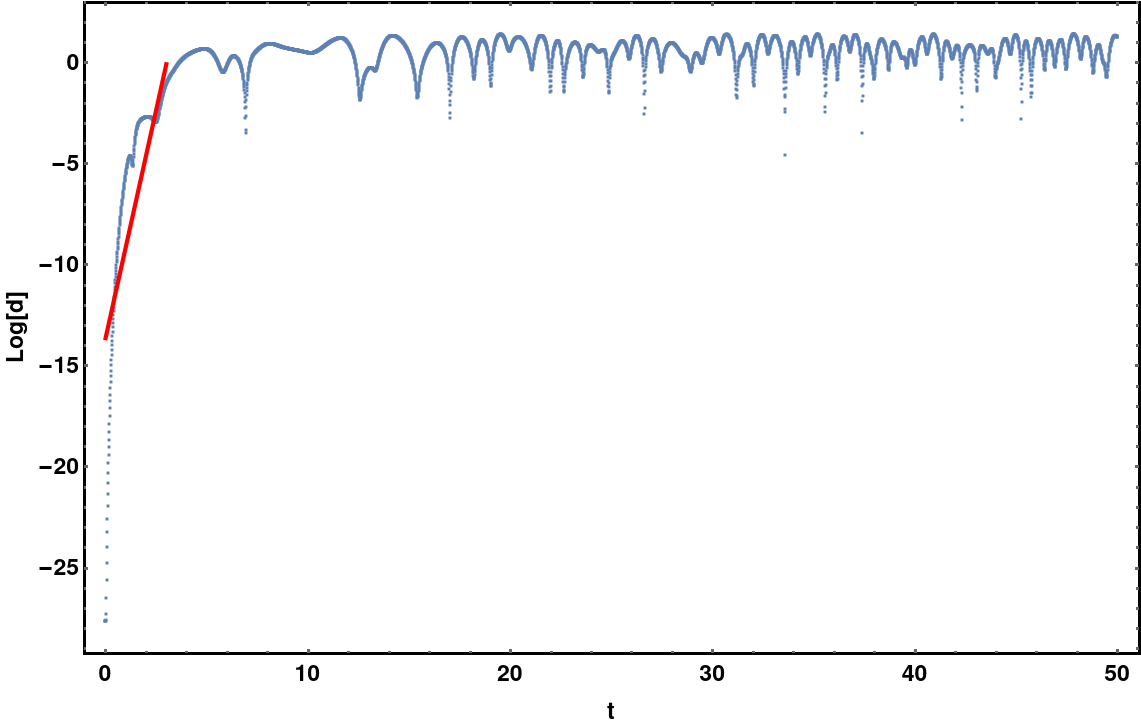
\includegraphics[width=0.9\linewidth]{double_pendulum_lyapunov}
	\caption{Exponential deviation between the trajectories of a double pendulum for slightly different initial conditions.}
	\label{fig:doublependulumlyapunov}
\end{figure}
%




% References
\nocite{*}
\printbibliography

\url{https://diego.assencio.com/?index=1500c66ae7ab27bb0106467c68feebc6}

\end{document}